\documentclass[a4Paper]{article}
\raggedbottom
\usepackage[margin=1in,footskip=.25in]{geometry}
\usepackage{graphicx}
\usepackage{xspace}
\usepackage{lipsum}


\usepackage{caption}
\usepackage{glossaries}

\usepackage{hyperref}
\urlstyle{same}

\usepackage{enumitem}
\setlist{leftmargin=*}
\setlength{\parskip}{12pt}
\begin{document}

\begin{titlepage}
%\setlength{\voffset}{-0.1in}
%\setlength{\headsep}{5pt}
%\setlength{\textheight}{650pt}
%titlepage
%\thispagestyle{empty}
\clearpage
\vspace*{\fill}
\begin{center}
%\begin{minipage}{0.75\linewidth}
    \centering
     
%=====================================================%
%---------------TITLE--------------------------%
%=====================================================%    
      
  {{\Large \textbf{Topic Analysis and Synthesis Report}\par}}
    \vspace{1cm}% 
     
%=====================================================%
%---------------Partial Fulfillment---------------------%
%=====================================================%
    \vspace{0.4cm}
    {
    \textbf{\large Software Project Management (SOEN 6481)} \par}
    \vspace{0.2cm}

%=====================================================%
%---------------Degree---------------------%
%=====================================================%

\vspace{0.5cm}
    {
    \textbf{\large Topic 123: Don't Elevate the Means Beyond the End} \par}
    \vspace{2mm}


    

%=====================================================%
%---------------AUTHOR'S NAME-------------------------%
%=====================================================%
\vspace{5mm}
    {\large by\par}
    \vspace{0.05cm}
    {\small {\textbf{Supradeep Danturti}}  (40226103)\par}

    \vspace{0.9cm}
    
%=====================================================%
%---------------Supervisor Name---------------------%
%=====================================================%    
%    {\Large \textbf{Doctor of Philosophy} \par}
%    \vspace{0.5cm}
    { Under the Supervision of \par}
    {\small \textbf{\textbf{Professor:{ Pankaj Kamthan}}}\par}

     

%=====================================================%
%---------------UNIVERSITY lOGO-----------------------%
%=====================================================%

\includegraphics[width=0.45\linewidth]{METRICSTICS/media/Concordia-university-logo.jpg}
%    \rule{0.4\linewidth}{0.15\linewidth}\par

    
%=====================================================%
%---------------DEPARTMENT'S NAME-------------------------%
%=====================================================%

    {\large \textbf{Department of Computer Science and Software Engineering}\par}
    \vspace{0.4cm}
%=====================================================%
%---------------DATE----------------------------------%
%=====================================================%
    
%    {\large {October 30, 2023}}
%\end{minipage}
\end{center}
\vfill % equivalent to \vspace{\fill}
\clearpage
\end{titlepage}

\tableofcontents 

\pagebreak
\section*{\begin{center}Abstract\end{center}}
The report delves into Seth Dobbs's thought-provoking article "Don't Elevate the Means Beyond the End," which scrutinizes the prevalent tendency within the technology industry to prioritize means, namely new technologies and processes, over the actual ends of solving business problems and achieving strategic goals. Dobbs posits that this inclination is largely fueled by a desire to continuously acquire new technological knowledge and a sense of detachment felt by development teams from the overarching success of their respective companies.

The analysis centers on two primary factors: the allure of embracing new technologies without discerning their direct alignment with business needs and the perceived disconnection between the development teams and the overall corporate success. Dobbs highlights how the eagerness to adopt new technologies sometimes overshadows the ultimate objective of addressing business challenges. This rush to implement the latest trends, such as microservices, serverless, or blockchain, often leads to a myopic focus on the means—implementing these technologies—instead of the intended end goal—solving business problems.

Moreover, Dobbs underscores the critical impact of the disconnection felt by development teams from their companies' broader goals. The resulting emphasis on what they can control, such as implementing new technologies, might steer them away from aligning their work with the company's strategic objectives.

The report provides comprehensive examples to substantiate Dobbs's arguments, illustrating instances where companies haphazardly adopted new technologies, leading to complex systems that were challenging to maintain and scale. It also highlights cases where misaligned Agile methodologies resulted in excessively bureaucratic and inefficient processes.

In conclusion, the report echoes Dobbs's assertion that genuine success emerges from a deliberate understanding of when and how to apply new technologies in solving business challenges rather than merely following trends. It advocates for a focused approach where companies comprehensively understand their business needs and strategically use technology to address those needs, emphasizing the necessity to avoid elevating means beyond the end goal.

The report amalgamates Dobbs's insights with industry observations, urging a recalibration in the industry's approach, prioritizing the alignment of technology and methodologies with actual business objectives for meaningful and successful outcomes.

\pagebreak
\section{Introduction}
The use of technology in businesses has become an integral part of modern-day operations. With the rapid advancement of technology, companies are constantly looking for ways to incorporate new technologies and processes into their operations to stay ahead of the competition. However, this has led to a growing concern where businesses are prioritizing the means (new technologies and processes) over the ends (solving business problems and achieving strategic goals). This issue is particularly prevalent in the technology industry, where new technologies and processes are constantly emerging, and companies are under pressure to keep up with the latest trends. As a result, companies may be investing in new technologies and processes without fully understanding their impact on business objectives.

\subsection{Motivation}
The motivation for this investigation is to address the growing concern about the impact of prioritizing the means over the ends in technology companies. With the rapid pace of technological change, companies are under pressure to keep up with the latest trends and innovations. However, this has led to a focus on adopting new technologies and processes without fully considering their alignment with business objectives. The goal of this investigation is to identify the root causes of this problem and provide recommendations for effective technology adoption that aligns with business objectives.

\subsection{Problem Statement}
The problem of prioritizing the means over the ends in technology companies can be stated as follows: companies are investing in new technologies and processes without fully understanding their impact on business outcomes. This has resulted in a lack of alignment between new technologies and business objectives, a waste of resources, and a lack of trust and confidence in the company's leadership. The problem is particularly prevalent in the technology industry, where new technologies and processes are constantly emerging, and companies are under pressure to keep up with the latest trends.

\subsection{Objectives}
The objectives of this investigation are to:
\begin{itemize}
\item Evaluate the Impact of Prioritizing Means Over Ends in Technology Adoption.
\item Identify Root Causes of Misalignment between Technology Adoption and Business Objectives.
\item Offer Recommendations for Strategic Technology Adoption Aligned with Business Objectives.
\item Propose Measures to Enhance Collaboration between Development Teams and Corporate Objectives.
\end{itemize}
\pagebreak

\subsection{}

\pagebreak
%\input{problem1.tex}
%\pagebreak
%\section{References}
    \begin{enumerate}[label={\textbf{Step}}]
      \item Item 1 \url{Item1.com}
      \item Item 2
      \item Item 3
    \end{enumerate}
%\pagebreak
%\strut \\
    \textbf{\large Contributions}
    \strut \\

    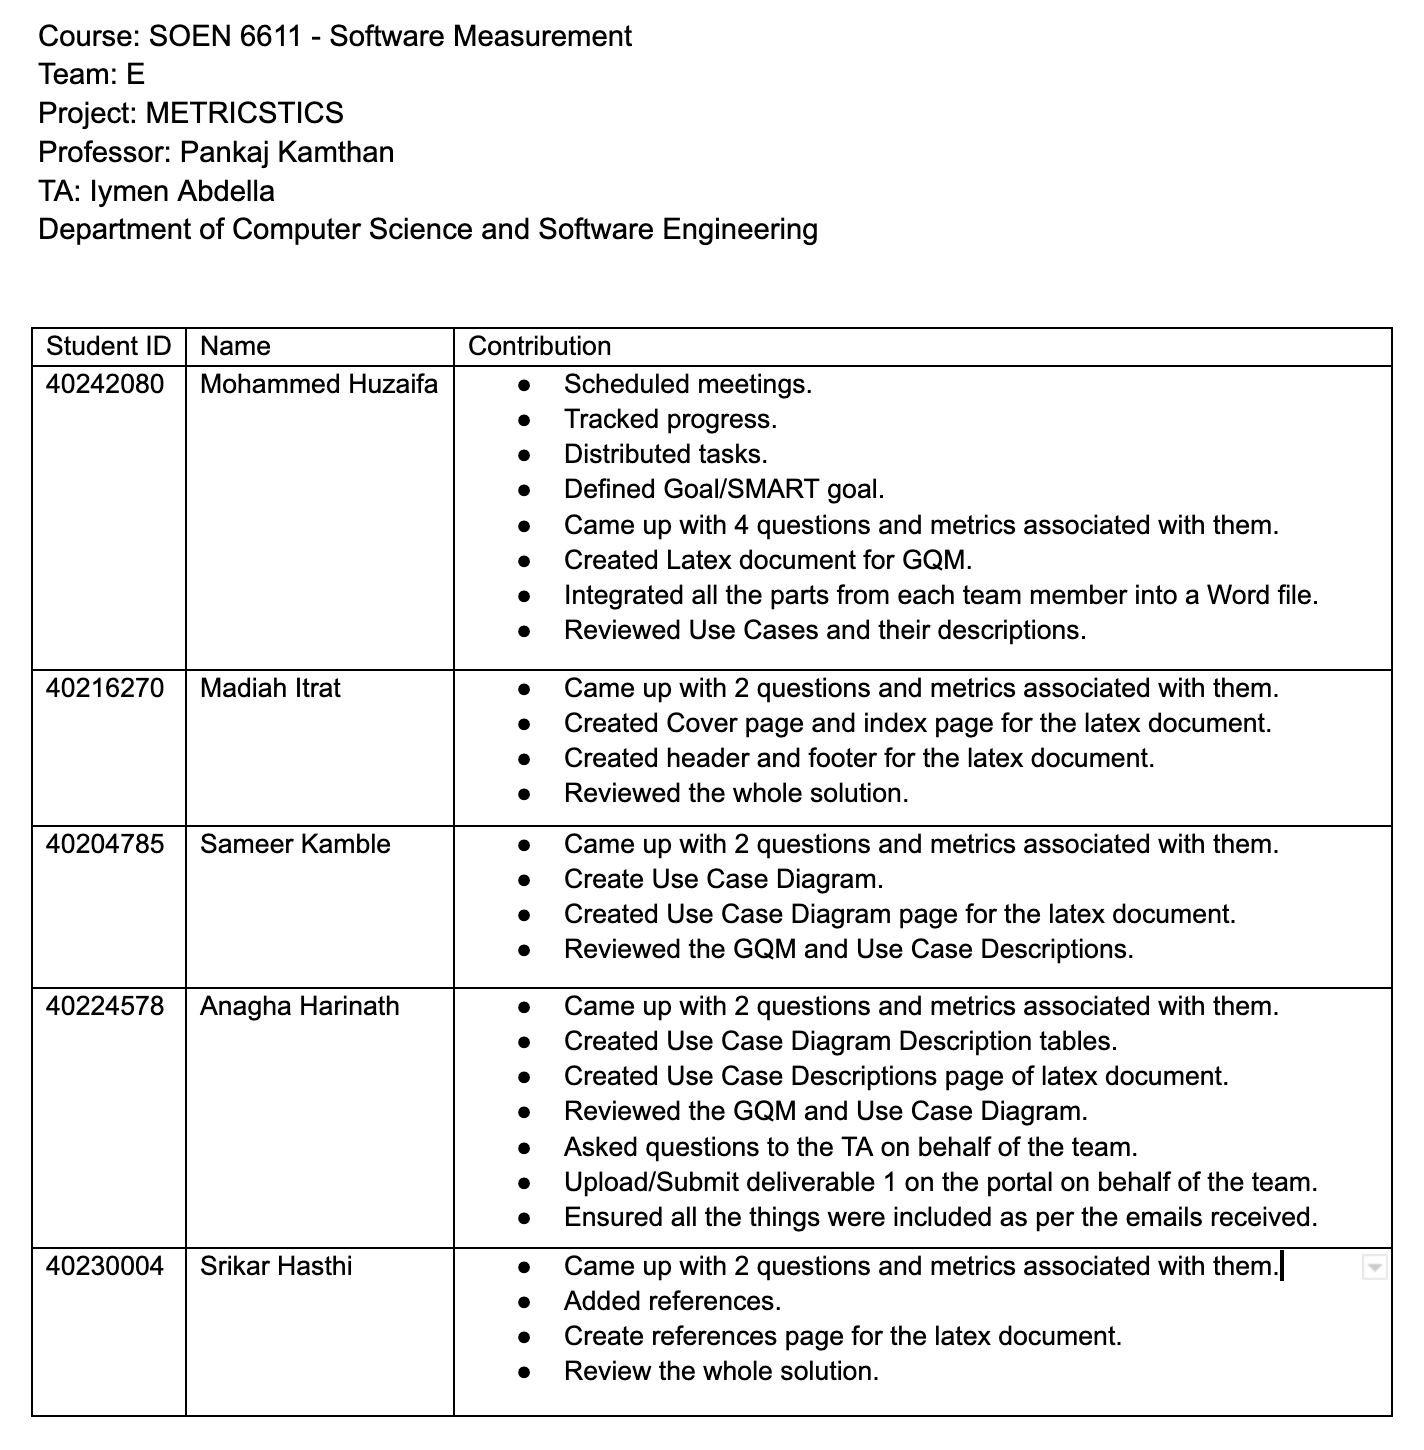
\includegraphics[width=6in,height=6.5in]{METRICSTICS/media/Contributions.png}

    \url{https://docs.google.com/document/d/1rRepmLwkqzTn-p66eA0qnV5Yr3qtT0x55YTpZvz9_jo/edit?usp=sharing}
    \strut \\
\end{document}